\chapter{Related Work}
\textit{In  this  chapter  we  will  discuss  theories and related work  that  address  the  topics  of  stress.  We  have  chosen theories  that  assisted  us  in  achieving  our  aim  which  is  to  understand  the  causes  and management  of  stress  at  the  workplace  in  particular  for people with stress disorder.  To  have  a  clear understanding of the Issue we have chosen the following theories; what stresses an individual and  an  employee, what  causes  stress  in  the  workplaces,  the  relationship  between  personal stress and job stress. What are the possible consequences and disadvantages of stress both to the  employees  as  well  as  to  organizations  and  lastly  the  different  approaches used  by  both employees to  manage  stress  are  discussed.  Afterwards  a  summary  and relationship between the theories is made a concept at the end.}
\vspace{5mm}

We have  decided  to  start  from  stress theories before explaining mental deficiency group because  we  wanted  to give  an  idea  for  the  reader  of what the main concepts are  and why  this issue is interesting. Therefore, knowledge of these concepts will lead the reader to have a good understanding as he / she reads the chapters and has a strong flow of ideas.  After  this  section we  go  on  to concept chapter to discuss how we conduct the study.

Also, This chapter will be presented the related work focused on workplace stress management and empowerment in the area of smart \ac{IoT} and human-computer interaction for the people with stress disorder.
\section{Stress}
Stress is a situation in which a person responds to or experiences something other than a new opportunity, the limitations and the effort that needs to be put in according to demand \citep{Naturale2007SecondaryField} . This stress situation can also be argued as a powerful state in which both the obvious result and the desired result are equally important and at the same time uncertain.

Nevertheless, the researchers carefully studied stress and realized that the stress state or the single term' stress' could either increase pressure and create tension that could be harmful in effect. If the stress condition becomes entirely unbearable, it can turn into depression and cause the person a traumatic crash; this situation is commonly referred to as distressed. 

Numerous scholars defined the term stress.Fletcher has given one of the definitions as  “Continuous process involving individual transactions with their environments evaluation of the circumstances in which they find themselves and attempt to resolve any problems that may arise"(Fletcher (2006) cited \citep{Rumbold2012APerformers.}). Stress is a condition in which an individual is under pressure and lacks sufficient ability to cope with it. Stress also suggests a direct negative reaction for both individuals and organizations, by damaging the original achievement of goals. (Table : \ref{tab:problem-stress}) Despite causing problems to the health and well-being of employees, stress also affects both the reputation of the organization and its productivity.  The negative side of stress can be observed as job dissatisfaction and unwillingness on the part of workers to their jobs, the reduction in the level of production and turnover and deficiency in the quality of work would be the company's demerits.

\begin{table}[ht!]
\centering
\caption[The problem of stress]{The problem of stress}
\begin{tabular}{|c|c|}
\hline
\textbf{The individual Threats to:} & \textbf{The workplace/organization:} \\ \hline
Health Well being/quality of life & Increased absenteeism and turnover \\ \hline
Functioning/goal achievement & Reduced quality and quantity of work \\ \hline
Self-esteem/confidence & Reduced job satisfaction and moral \\ \hline
Personal development & Poor communication and increased conflict \\ \hline
\end{tabular}\\
\footnotesize Source: \citep{Michie2002CausesWork.}
\label{tab:problem-stress}
\end{table}

A study by \citep{Michie2002CausesWork.} has stated that workplace employees are a victim of stress; this phenomenon has affected both employees and employers.  For example, the reasons for employees are disability, early retirement, burnout and unmotivated, etc., and for employers, the stressful thing was the loss of staff, reduction in turnover, dispute, consumer dissatisfaction economic threat and major difference between realistic expectations and performance.

Stress is sometimes described in the emotional framework, and it can be caused by uncontrolled emotions. So we thought about discussing emotions and stress in the next section in order to find out the interlinked points between stress and emotions. 

\subsection{Emotions and Stress}
If  stress  is  described  in  the  framework  of  emotions,  it  seems  to  be  quite  complicated  and difficult  to define  due  to the  unavailability  of  a  pure  and  exact  definition about  emotions. Emotions refers to a person's’ subjective feelings and moods, it states a complex changes in physical  and  psychological  situation  of  an  individual  that  affects  thought  and  behavior. Anxiety, depression, frustration, and humiliation are ultimately the product of stress emotions. Anxiety is known as one of the worst emotional factors in a person's behavior which causes many incurable problems and disorders. Emotion reaches an intense human behavioral force that leads to a condition where one can not make better decisions or act normally. The researchers and psychologists divided the emotional hypotheses into various categories: physiological, psychological, and cognitive.  Emotional theory physiological refers to the body's signal or reaction.  Neurological suggests brain reaction to the emotions. A cognitive theory explains the roles of thought, or the functions of the brain in emotional development \citep{Ashforth1995EmotionReappraisal}.

Stress is described as "the psychological, emotional, and physiological responses of the body to any demand perceived to be threatening the well-being of an individual" \citep{Bloisi2007ManagementBehaviour}. Whereas Lazarus ' stress is described as a "process of evaluating events or circumstances as dangerous, threatening or challenging to determine possible responses and react to such events. Cited in Lazarus, 1993 \citep{Bloisi2007ManagementBehaviour}.Stress gives both positive and negative reactions to our actions because our rational assessment and assumption of stressors make a difference in how we react to and how we deal with the issue that is perceived as stressors.

The stress is constructive and destructive. Constructive stress is the anxiety feeling which makes us perform well in our daily lives. Stress could also be the motive force for testing ourselves and encouraging us to do something. Although disruptive stress has an unintended consequence of stress known as distress \citep{Bloisi2007ManagementBehaviour}

Our main purpose of this study is to understand the causes and treatment of stress disorder from the point of view of individuals with mental disability. Therefore we will be discussing on the basis of what stress is and the different stress indications that would help us to clear the way to finding the causes and stress management.  It will also be a helpful guide to help the reader gradually follow The next segment addresses the various stress symptoms.

\subsection{Symptoms of stress}
Some of the stress symptoms described in \acs{CIPD} state that people who are stressed tend to increase their consumption of alcohol and smoking. It may also be noted that stressed people often find it difficult to get a good night's sleep.  Increasingly, the stress-related issues have turned into a major problem for both employers and employees. The stress symptoms are explained in (Table \ref{fig:symptom}) and reflect the stress symptoms from the mental, behavioral and cognitive perspectives.The behavior of the people, or more specifically changes in the behavior of the employees, will show the sign of stress. Whereas in the areas of feelings that lead to prolonged acute health problems or diseases such as anxiety, irritation, fatigue, rudeness, and depression, the sign of stress to people can be sensitive in different ways.

\begin{figure}[ht!]
\centering
\smartdiagram[constellation diagram]{
    Physical \\symptoms,
    Stomachache,
    Sweating,
    Muscle tension,
    Headache,
    Rapid \\breathing,
    Shaking,
    Frequent \\urination,
    Stop Talking,
    Fast \\heartbeat,
    Trouble sleeping
}
\captionof{figure}{Stress disorder Common physical symptoms}
  \label{fig:symptom}
\end{figure}

Feelings such as nervousness, fatigue, frustration, and dissatisfaction are seen as emotional symptoms, which can be associated in people who feel stressed and behavioral indicators that can be seen with employees who make performance errors, sleep difficulties, confrontation with colleagues, and less social. 
The symptoms of cognition are that it would be difficult for a stressed person to be attentive to his task, and find it difficult to memorize details as well as being passive and absent from situation.
Our body also shows signs when stressed signs such as as being out of breath, sweating most of the time, heart pain, skin rashes, etc. are the physiological signs of stress to the body. The lack of treatment for these particular problems can lead to further difficulties in mental and physical health conditions such as heart disease, depression and anxiety as shown in Table \ref{fig:symptom}.

%mix with upper table symtoms
Stress can produce both physical and psychological symptoms. People experience stress disorder differently. Common physical symptoms shown in Figure~\ref{fig:symptom} 

Stress disorder can cause mental or emotional symptoms in addition to physical ones. These can include: Figure~\ref{fig:mentalsymptom} 
\begin{figure}[ht!]
\centering
\smartdiagram[descriptive diagram]{
    {feelings,impending doom},
    {panic,panic or nervousness},
    {difficulty, concentrating Special},
    {irrational, anger},
    {Mood swings, unaccountable change of mood},
}
\captionof{figure}{Stress disorder mental symptoms}
  \label{fig:mentalsymptom}
\end{figure}

\subsection{Different level of stress and symptoms}
Many people may be unaware that there are different kinds, but based on study we have categorized stress into four types : acute, episodic acute, and chronic . 

And if we are feeling stressed, it can be helpful to know which type we are dealing with.Different level of stress is shown in the figure~\ref{fig:levelOfStress}.

\begin{figure}[ht!] % supposedly places it here ...
  \centering
  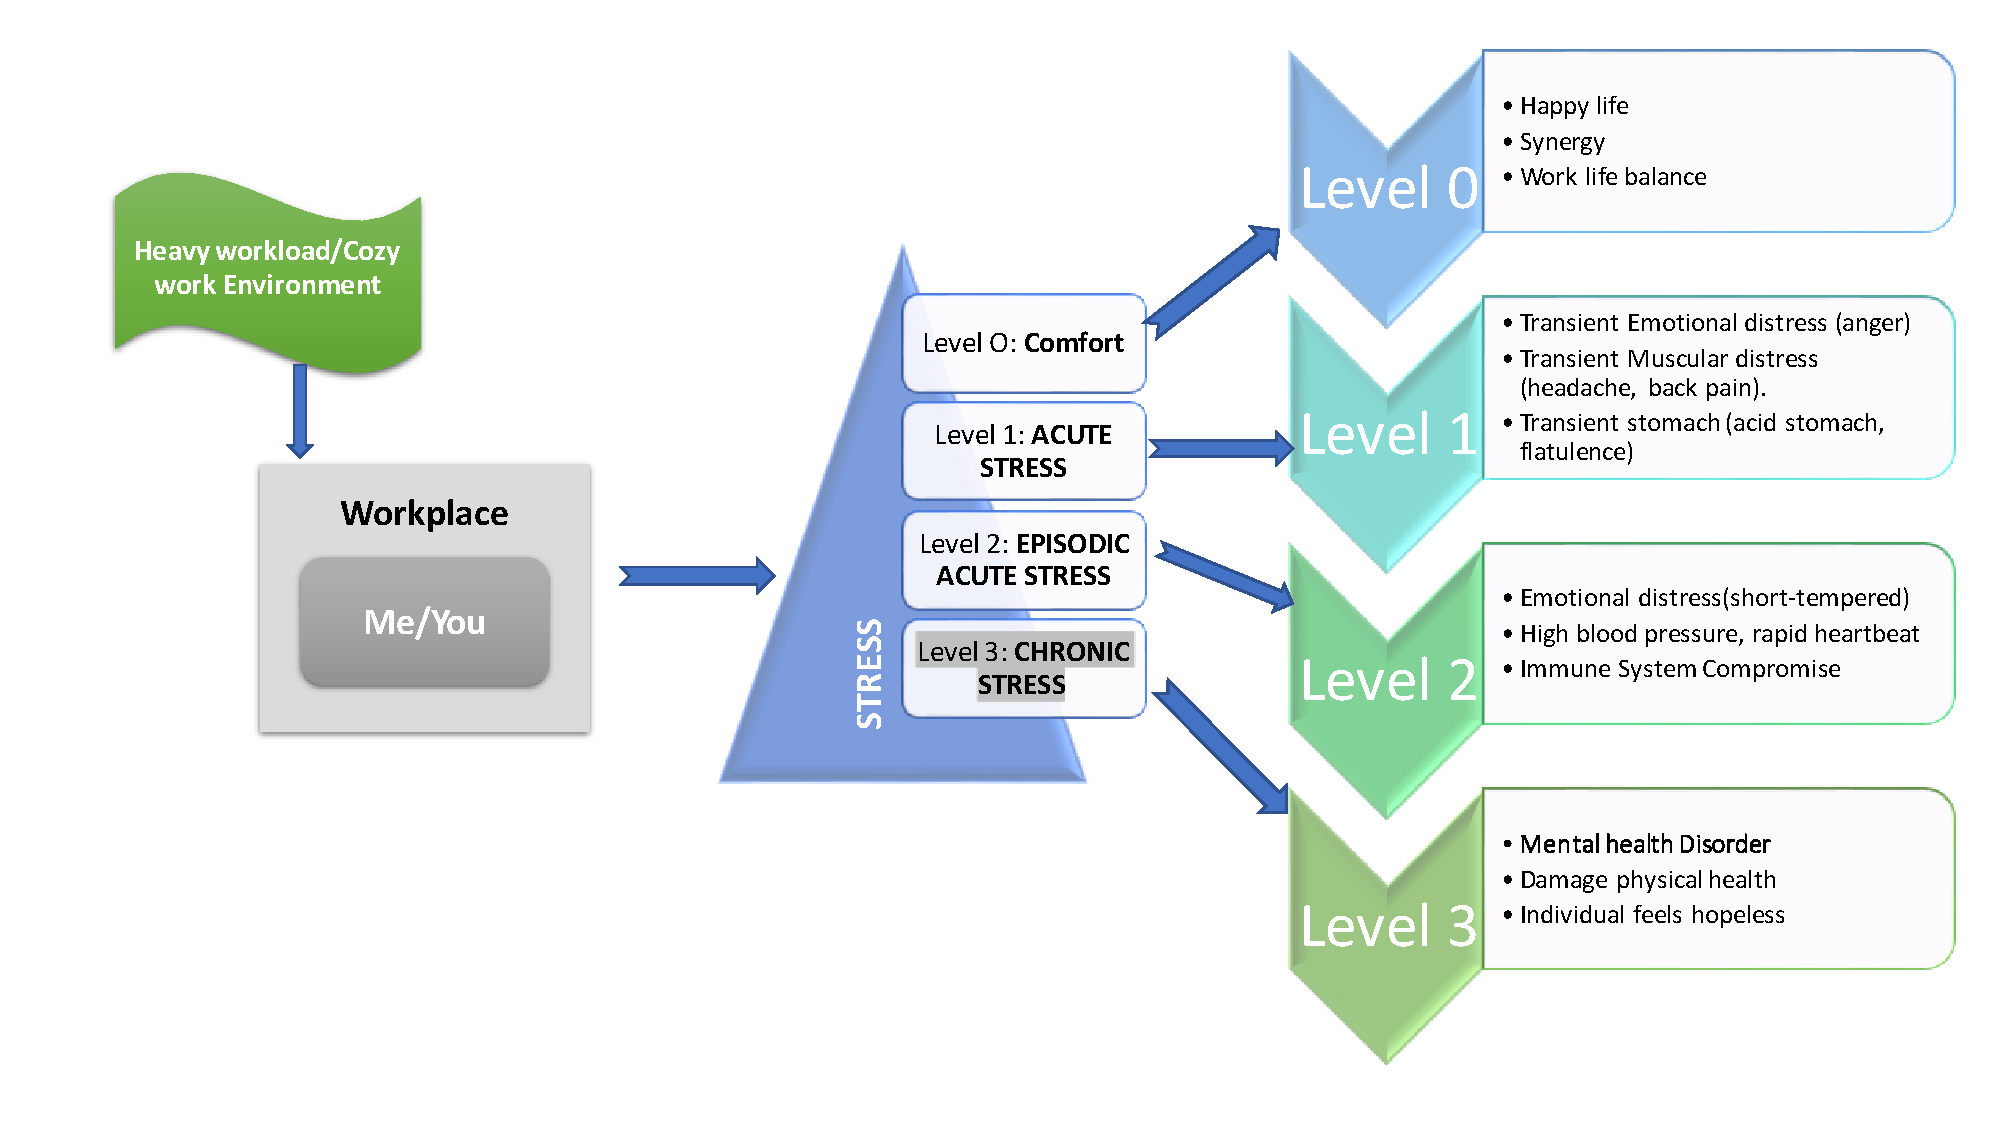
\includegraphics[width=1.10\linewidth]{chap1/images/problem_goal.pdf}
  \caption[Different level of stress ]{Different level of stress with problems.\index{Hasnain}}
  \label{fig:levelOfStress}
\end{figure}

\textbf{Comfort Stress}

Psychologists refer to as "Eustress," is the sort of stress that we feel when we're excited. Our pulse is overeating and our hormones are springing up, but there is no threat or fear. When we ride a roller coaster, compete for a promo, or go on a first date, we feel this type of stress. This good stress has many triggers and it keeps us alive and excited about life.

\textbf{Acute Stress: }

A close call on the street, or speaking before a large crowd, are the kinds of conditions that could cause acute stress. The symptoms are physical, emotional, and/or behavioral but they are usually short-lived.

\textbf{Episodic Acute Stress: }

Episodic acute stress occurs when someone gets frequent bouts of acute stress. People with this kind of stress will oftentimes take on more responsibilities and projects than they can handle. They may seem like they’re constantly in a rush, always running late, and are disorganized. People with episodic acute stress can also be hostile towards others and have strained relationships.

\textbf{Chronic Stress: }

Chronic stress happens when people feel trapped in a bad situation. Whether it's an over-demanding job, an unhappy marriage, or a dire financial situation, this is the kind of stress that starts to wear away a person's physical and mental health significantly.\citep{Cottini2013MentalEurope}

So this section of recognizing stress symptoms should be the first step in understanding whether or not an employee is anxious at the workplace.  Only then can one go to better understand the causes and the letter about better Stress management mechanisms. We now start with personality types or group of people and then types of stressors in order to have a logical flow of hypotheses before we get to the key theories of this study which are causes of stress and stress management.

\section{Disability Group}

\subsection{Types of personality and the degree of being affected by stress} 
A research by Friedman \& Rosenman (1974) established two personality traits they named personalities of type A and type B.  

Type A personalities are prone to stress because of the pressure they put on themselves, they are constantly trying to multi-task, they are violent and nervous. Whereas the personalities of type B are more calm and relaxed.

Due to the hard work type A personalities put into their careers they are more likely to be promoted and have control over their career, but they are also the ones that are likely to be reported to have too much stress or suffer from health issues. And the suffering people with such characteristics never get to the top of corporate hierarchy because of frustration and lack of patience.

While type A personalities are much better in comparison with type B personalities, type B personalities are much stronger and have the potential to become top executives. Consequently, thoughts of a person depend on how he / she perceives a situation as stressful or not.  Mostly it depends on the temperament of a person, and the level of stress encountered is also influenced by the individual characters of individuals. \citep[p.314]{Bloisi2007ManagementBehaviour}

According to \cite{LazarusR.S.Folkman1984StressCoping.} the degree of stress encountered depends on factors such as market awareness which means that people need to know that there is demand. If people try to satisfy their demand, they might be harmed in the event they don't respond appropriately. Firstly, the threatening situation must be of interest to the individual and consequently the consequence of the demand must be unknown. \citep[p.310]{Bloisi2007ManagementBehaviour}

\subsection{Types of stressors}
Below are stressors which affect an employee in the workplace. 

1, Work role: -this happens when the employee is uncertain as to what job he / she should be doing or when the employee has an enormous amount of work to do with such a short amount of time. Stress may also grow as a result of uncertainty.  This situation will probably occur at any form of occupation.

2, Underutilization: -This means that the worker does not have enough work to boost his / her motivation.

3, Responsibility for others:-This increases the level of stress if workers are faced with high responsibility for others.  Those who are in charge of others at the workplace and those higher up the corporate hierarchy are often vulnerable to greater stress because of their co-workers' expectations.

4, Poor working conditions: -these factors also contribute significantly to stress, which include extreme heat, cold, noise and overcrowded. \citep[p.318-319]{Bloisi2007ManagementBehaviour}

\subsection{Job anxiety and employee Relationship}

Firstly, we use below mentioned equation to estimate the relationship between task anxiety and employee, career and workplace characteristics:

\[JA_{i_j} = X_{i_j} \beta+Z_j \gamma+\epsilon_{i_j}\]

Where \(X { I_j}\) refers to employee's personal and job-related characteristics \textit{i } in the workplace \textit{j } and includes age, gender, race, impairment, highest academic qualifications, part-time employment, temporary employment, occupation, supervisory duties, whether individuals perceive themselves to be over-skilled or under-skilled, and whether they perceive themselves to be over-skilled or under-skilled. Workplace level controls \(Z_j\) include sector, workplace size log, area, existence of an appraisal system within the employee's occupation, and workforce composition (female, age, temporary, full-time). They also account for organizational change (reported by the manager), performance-related compensation, team work prevalence and training receipt.  In addition to these more traditional controls, it is also important to include a measure of co-worker anxiety that was not used in previous studies but could capture common unnoticed effects on the workplace and spillover effects among workers, the latter being noted \citep{Cottini2013MentalEurope}.

\section{Causes of stress}
Employees undergo and feel stressed due to a set of different factors and therefore the occupational stress reactions are not a separate thing. \citep[p.8]{Fairbrother2003WorkplaceSatisfaction} Increasingly, the level of stress among employees is changing rapidly due to a variety of reasons such as work exhaustion, overcrowded workplace, generating noisy machine noise and arousing tensions between employees and employers as a result of poor or inadequate decisions.

Stress may emerge from changes that are made in our personal lives.  Personal issues that lead to stress include family issues such as loss of loved ones, financial problems and divorce.  These can be categorized as individual triggers which lead to stress.  On the other hand, stress is also triggered by organizational factors which are those faced by the workers at the workplace.Issues such as task uncertainty; that is not being able to know exactly what we are supposed to do and what others expect of us and also having too much work at hand with too little time to do it can cause stress at the workplace.  Certain organizational stress factors are poor working environments in which the employee is often too busy, where noise, cold or too warm temperatures are present, and in which the office is often filled with people rushing about.  Whereas problems that lead to stress are lack of control, suddenness and uncertainty; position ambiguity in particular is the primary cause of stress at work. \citep[p.350]{Parker2008PersonalityProcess}

Many organizational variables which can be considered stressors often rely on job types and work requirements.  They play an important role with respect to stress issues, for example if the task is high-stressed or not.  High stress jobs are the kinds of jobs that take plenty of time and put the workers under the work pressure. It is also notable that workers frequently suffer from poor working conditions, if the job is carried out in an uncomfortable atmosphere \cite[p.317]{Bloisi2007ManagementBehaviour}

In  order  to  study  in-depth  the  main  reasons  of  stress  or  why  the  employees  feel  stressed specifically at the workplace, we have described some main factors in the next section that often initiates stress.

\subsection{Workplace factors causing stress}

Scholars have identified a large number of occupational life characteristics as being related to stress.  Workers feeling the stress reaction at the workplace are not a new aspect. Spark \& Cooper (1999) reported their research by performing a retrospective survey of 7,099 workers from 13 different businesses and jobs.   They identified a significant statistical assembly between factor in the workplace and negative health symptoms or mental condition disorder such as anxiety, depression and irritation.

For the following reasons employees usually feel stress at their work.
\begin{enumerate}
    \item Work overload
    \item Misuse of power
    \item Inadequate decisions or leader behaviour
    \item overcrowd, noise
\end{enumerate}


Work and job is itself a stressful phenomenon and is therefore related to stress by various aspects (Defrank \& Ivancevich, 1998; Spark \& Cooper, 1999; Taylor et al., 1997). According to Burke (1988), the factors associated with roles in a work environment are Nilsson \& Burke (2000), namely the presence of low-level authority, arbitrary role or conflict over the position. We add that stress is associated with that physical conditions at the workplace including concurrent permanent noise, overcrowding and lack of confidentiality. Leader's or chief's actions can also influence stress level \cite[p.9]{Fairbrother2003WorkplaceSatisfaction}

\subsection{External Factors of stress}

From an individual perspective as well as in the workplace, we explored the causes of stress. There we concentrate on potential stress factors for both staff and organisations. Employees will be directly affected by external stress factors but corporations are often indirectly affected.

According to the Kirkcaldy \& Martin (2000) report, workers have endured tension because of various reasons. There has been primarily tension associated with important issues, including environmental and economic aspects.   Corporate atmosphere and workplace implications of work contentment, corporate commitment and employee behavioral elements are included in the environmental factors.   For example, in hospitals dealing with wound, death and dying on a regular basis remarkable occupational atmosphere for doctors and nurses. \citet[p.10]{Fairbrother2003WorkplaceSatisfaction}

External factors outside employee and organisation's influence are based on political dynamics and economic factors.  Some of the economic consequences for a business that concerns workers are economic risks such as retirement and downsizing. Changes in political situation or economic hardship are out of the reach of workers, therefore the possibility of retirement and downsizing in some way affects employees. \cite[p.320]{Bloisi2007ManagementBehaviour}

Technological advancement is also another external factor which has largely contributed to productivity. This caused a remarkable decline in labor demand on the market which had an impact on job security for the employee. Although familiarizing oneself with new technologies is necessary, it can be considered stressful if it is viewed as difficult or hard to know. New software may cause stress among employees due to technological changes such as computerized systems. Politics is also an important stress factor, in addition to technological changes. Will render the workplace more difficult in situations where there is significant shift in government policy or employee mistrust against government.  \citep[p.309-320]{Bloisi2007ManagementBehaviour}

A study conducted by Rees (1995) and Young \& Cooper (1995) reported that many research findings and adequate knowledge are available in this particular area. Scholars can not directly apply all of their results to all workplaces because the factors in the workplace are not always linked to stress at specific workplaces or, in other words, stress factors are not always stable, consistent and common to a group of occupations. This ranges from environment to environment, work to work or situation to situation but on the team being surveyed the relationship differs between stress and job satisfaction.  \citep[p.  8]{Fairbrother2003WorkplaceSatisfaction}  

Next, we address stress in a specific context of work to see what can cause stress and identify the roots of the problem in one definite environment of employment.
%09.02.20
\subsection{Stress in a specific job context}
Royal Australian Navy performed an internal staff study on what causes a seagoing ship to be stressed out. (Royal Australian Navy 1996).It defined employees as suffering from stress because of the following different reasons. The survey shows that 35\% of employees working on ships and 25.9\% of regularly employed officers are stress associated with their job. They mentioned a few reasons related to their stressful occupation such as limited work environment situation and living conditions on a seagoing ship. As an unpleasant and restricted situation due to working in an isolated community, respondents demonstrated their salient aspects linked to their stressful work, career, and working environment.  Naval officers, on the other hand, are under pressure because of restrictions and strict schedules that shorten their access to regular personal routine and even interrupt the sleeping time.  Gilks \& Buckley (1995) commonly reported that 50\% of officers are shortening their personal duties to gain time for broken sleep.

It relates to our goal of connecting the causes of stress, whereas here the causes are that the working conditions are beyond employee control and have a negative effect on the employee's\cite[p.~10]{Fairbrother2003WorkplaceSatisfaction}.

By reading this section, the reader has grasped an understanding of the potential causes of stress in personal life, in the workplace, as well as the external factors outside employee and organization control.  So now we can continue to see what potential effects, consequences and drawbacks stress can have on workers and on the company as well.

\subsection{Consequences of stress on employees}
Employee stress consequences Episodic stress is characterized as "a pattern of high stress followed by relaxation periods" while chronic stress is defined as "stress caused by the continuous interaction of stressors without relief \citep[p.313]{Bloisi2007ManagementBehaviour}”The consequences of suffering from adverse chronic stress are divided into three categories: physiological, psychological, and behavioral. Some of the signs of physiological stress are blood pressure, high heart rate, and headaches while psychological symptoms are nervousness, unhappiness, and bad tempered ness all of these emotions can result in lack of concentration, indecision, and absenteeism. If individuals can not find solutions to their stressors they may end up feeling depressed, insane, and often refuse to believe in being caught up in an imaginary life. Higher alcohol intake, aggressive attitudes, and restlessness are the behavioral consequences of individuals subject to chronic stress \citep[p.323]{Bloisi2007ManagementBehaviour}

Another consequence of stress is that it can cause a lot of illnesses.  There is evidence that stress may be one of the causes of these diseases; coronary heart disease, hypertension, and cancer, but the degree to which one person is affected by a stress-related disease often greatly depends on what kind of personality that person has, i.e. if that person has type A personality or type B personality.  (Friedman  \&  Rosenman  (1974)  Also  Friedman  \&  Ulmer (1984)describe Type A personalities as competitive, punctual, easily frustrated and perfectionist, whereas Type B individuals are relaxed, sensitive and satisfied with their job and are less prone to stress.

A transition in physiological, psychological, and behavioral improvement could therefore be considered a consequence of stress.  Generally, blood pressure, depression, elevated heart rate etc. are the physiological effects of stress, while the physical consequences are chronic stress causing absenteeism, indecision, nervousness, etc. Sleeping problems, elevated alcohol and smoking habits, frustration, and so on, are the behavioral effects of stress. Confronting the situation is some of the reactions to behavioral stressors. There are two words to be taken into consideration when coping with stress. The first is known as (fight) to address the problem or dilemma and find a solution to it and the second is named (flight) to walk away from the stressors. \citep[p.348]{Parker2008PersonalityProcess}
%10.02.20
\subsection{Disadvantage of stress for employers and employees}
Stress has several adverse effects on the workplace's employee occupational functions. The negative effects include lack of willingness and interest in work, decrease in productivity, reduction in performance, and poor dedication to the company, job and colleagues.  It also increases the level of rigidity and inflexibility related to job performance and provides a space for confusion or disrespect for the organization's laws, policies and regulations. \citep[p.10]{Fairbrother2003WorkplaceSatisfaction} Depending on the management perspective, stress problems can be examined in two ways, stress risks to workers within the company and direct stress impact on the workplace / organization. 

\subsection{Steps towards Stress Management for employees and organizations}
Productive stress management requires three phases for both workers and organisations. 

1, Awareness: it helps to understand when efficiency and absenteeism are declining.

2, Cause determination: Find out what causes this suffering and its effects.

3, Do something constructive: Seek solutions to problems that exist

At one stage tension could be viewed as an unavoidable state. Maintaining productivity complicates the situation and also disturbs having good work and social life. The first step towards stress management is to recognize signs of stress, such as anxiety, frustration, irritation, etc. Upon identifying these symptoms, the next step is to find out the causes and work out their impacts. The third and final step is handling a stressful situation effectively.

There are two types of coping mechanisms proposed by Folkman and Lazarus (1988) the first is that the stressors are either modified or completely removed (problem focused) here. The second mechanism is (emotion-focused) where workers learn to adapt to circumstances, and also cope constructively with stress.  The difference lies in where the stressor is specifically confronted in problem-focused coping mechanism; it is either changed or eliminated. Whereas in emotion-focused it is only the people who change or learn to adapt productively to the stressor. \citep[p.326]{Bloisi2007ManagementBehaviour}

The first person in control (charge) of managing stress eventually rests on the employee and the following are some of the techniques to cope with stress in relation to the workplace.

1, Time management: plan tasks accordingly, efficiently managing one's time, prioritizing tasks to be dealt with first. Efficiency and efficiency are respected here.

2, seeking help: Staff, co-workersor supervisors are encouraged to receive assistance to improve the performance.

3, Emotion-focused strategies: as discussed previously, it is important to learn how to respond to stressors in a positive way. Popular approaches based on emotion include exercise, companionship, relaxation and leisure activities. \citep[p.328-333]{Bloisi2007ManagementBehaviour}

\section{Employees stress management at the workplace using Smart \acs{IoT}}
In most situations, the staff and organizational strategies try to reduce the threat to the health of workers in their workplace associated with stress.  Specific strategies involve many methods, such as workplace, physical and psychological seminars, routine instruction, consulting counselors, etc., to reduce the risk of stress associated with employee health. The exact purpose of these consultations and activities is helpful in helping workers become aware of the available resources.

Existing services and tools help employees improve their skills and abilities against challenging circumstances, or alter their current situations. (E.g. physical, psychological, occupational). A wide variety of training courses are offered to help employees improve their skills.  (e.g. effective or sufficient management, time management, communication skills, assertiveness, problem-solving etc.). Both behaviors lead to higher work performance and positive employee performance toward stress and coping with it. 

Training helps workers illustrate the following features:
\begin{itemize}
    \item One can understand the signs of stress 
    \item Gains versatility in behavioral patterns, and when it begins, one can participate in the stress cycle. In a typical situation tension usually grows slowly. More tension brings more trouble. 
    \item It allows situational awareness and offers a plan of action to reduce stressors.
    \item Develop ways of effectively reacting to stress and the correct coping mechanisms. 
    \item Learn coping skills, motivation skills, and improved self-confidence.
\end{itemize}

The above methods have proven helpful in managing stress or in preventing increasing stress. (Michie, 2002, p.69-70)

\subsection{Smart \acs{IoT} for Stress management}
%need Rephraise
Over the past few years, \acs{IoT} technologies have been widely applied in various health fields through many initiatives. \acs{IoT}-based devices, such as mobile phones and wearable computing, are often used in the field of health metric self-measurement.  These tests are used to promote health, well-being and stress management where improvements in critical parameters can be observed and play a role in changing human behaviour. 

Various types of wearable and sensors used individually and in combination, are designed to track vital parameters that indicate stress or arousal symptoms, such as heart rate, GSR (galvanic skin response), blood pressure, and others. 

Heart rate is one of the markers of health status, a reflection of the presence of anticipation.  Heart rate monitor is commonly used in sports equipment\citep{Fu2015SystemDevice} and fitness.  The heart rate sensor will boost the detection of stress levels in daily life and help to provide stress management\cite[p.330-339]{Millings2015CanTechnology} \cite[p.361-371]{Parnandi2017PhysiologicalGames}.

Smartphones play a large part in managing stress.  Some apps have embedded sensors to detect and track stress-or depression-indicating behaviors\cite[p.175]{Saeb2015MobileStudy}. Others introduced biofeedback, i.e. stress and anxiety therapies\cite[p.1274-1286]{AlOsman2016UbiquitousManagement}\citep{Zafar2017PlayingBiofeedback}. Ahtinen proposed a mobile stress management application that includes four mental wellness-training intervention modules\cite[p.11]{Ahtinen2013MobileStudy}. The study, which recruited 15 university participants, has shown significant improvements in respondents ' stress and life satisfaction.

One consumer stress management system is Biosync Technology. The heart rate of the patient, the galvanic reaction to the skin and the gestures are measured. Data are processed automatically to assess the stress level of the patient and, in turn, preventive measures are given to ensure a better life\citep{Nishida2017BioSync:Experience}.

A number of papers investigated the assessment of the psychological condition and physical reactions in students\citep{Santos-Gago2019InnovativeReview} and their academic success, as well as the estimation of their correlation, or the improvement of the mental health of students. Shen, Wang \& Shen's research \citep{article} used psychological cues to predict emotions.  In the research cycle they explored the existence of different emotions and suggested a sensible e-learning model. The data were collected using three sensors: the skin conductivity sensor measuring electrodermal activity, the blood pressure measuring photoplethysmograph sensor and the brain activity measuring EEG sensor. In the natural environment, measurements were taken over several weeks on one subject, as close as possible to the daily environment.

In this research we want to design and implement a system to identify the psycho-physiological signals that signify stress in the workplace during work. Some research uses different types of devices to understand occupational tension, but few of them cope in a real environment with stress management. Our goal is to provide a solution that would validate stress feeling and help employees manage their stress during work.

A mobile application with the relaxation material will reduce employee anticipation and have an effect on stress reduction during work.
\section{Summary of Related Work theories}
To sum up the theoretical chapter and the core theories discussed in this section, stress, causes of stress and the management of stress with each core theory including subtopics such as symptoms of stress, personality types, factors of stress, workplace factors causing stress, types of stressors, consequences and disadvantages of stress on employees and organizations, employees stress management and organizational approaches to stress management were discussed.
%10.02.20 evening

This chapter tarted off with the presentation of what stress is and the definitions provided on this subject by various scholars.  Some of the stress symptoms were addressed with a view to defining a condition as stressful. Our research seeks to explain why and how stress is handled. We addressed the various causes of stress, because the probability of being affected or the likelihood of perceiving a situation as stressful depends largely on the individual's personality. Further the disadvantages and consequences of stress have been described for employees and the organization in order to achieve productive stress management.

To have an effective stress management system one should be able to know the causes of stress and how it will affect the workers, and then address its implications.  Therefore, after looking at the effects and causes in the workplace, we saw the strategies used to minimize the negative impact of stress from both the viewpoint of the workers and the management of human resources.

The theories chosen are important to our intent, because they were chosen from the beginning to tackle the stress problem that starts from defining what stress is. In doing so, it clarifies what we are going to be talking about to readers from the start and the reader wouldn't have to turn to other sources to understand the concepts by our paper as they've been clearly stated and clarified enough.  The theory of causes of stress is important for our research to understand whether the causes of stress are linked to personal or work. This fulfills our goal of recognizing what causes stress in both employees and management. Since recognizing the causes of stress, we decided to find out how to manage stress from the viewpoint of both the employee and the management.

The inference in relation to our intent which can be drawn from the hypotheses is that the causes of stress in the workplace are job fatigue, poor working conditions such as overcrowded working conditions and noise.  And the stress of Employee can be managed through proper time management, seeking help from \acs{HRM}. The emotion concentrated on activities such as recreation, companionship, and exercise. Management plays an important role in determining and controlling the stress level of workers in the workplace and should use various methods to reduce stress such as implementing training courses to assist the skills of the employee, providing a better working environment and ensuring that employees receive adequate feedback and advice when necessary. The description is the method we will be evaluating the data from.

Now that the reader has an understanding of what stress is and why we find this topic fascinating we would now like to go on to the next chapter that is the design chapter, discusses how we perform requirement engineering and persona analysis for this report.